\section{Global overview}

The overhall principle of the website mycustom is resumed on Figure \ref{fig:principe}. The main page of the website is organized as a single app page. The link between the database and the interface client is done by several Django App namely \texttt{"home", "collection$\_$ephemere", "cutsomise", "achetez", "vendre"}. These apps contains the HTML templates that render in the interface client and the Django model used to fulfill them. The interface admin is able to modify the database in the backend and thus the interface client. In order to fully understand how a Django app works, see \cite{Django}. 

\begin{figure}[!ht]
	\centering
	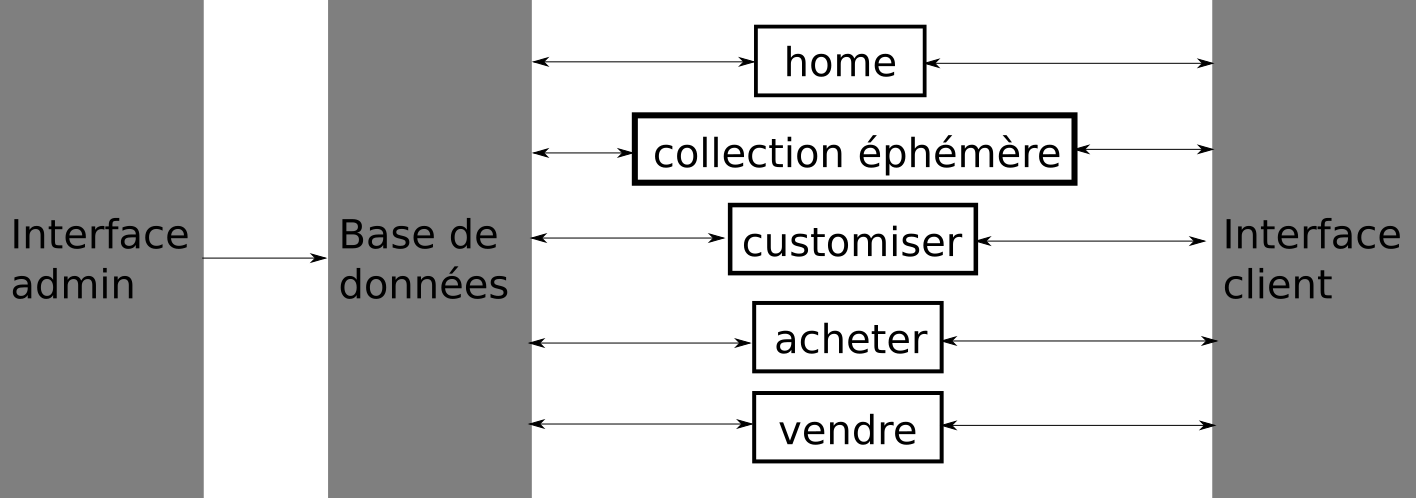
\includegraphics[width=0.5\textwidth]{Intro/principe}
	\caption{Global principle of the mycustom website}
	\label{fig:principe}
\end{figure}

The purpose of each of theses section is the following : 

\begin{itemize}
	\item \texttt{home} : Contains the landing page of the website, i.e the first thing that the client see. The Django app contains a video for the welcome page, the HTML template for the header, the footer, the menu and the welcome page. The Django models contains all the visual characteristic for the welcome page
	\item \texttt{collection$\_$epehemere} : Contains the transitory trends, i.e textile and logo of the month. The Django models are the \texttt{collection$\_$Ephemere} that contains all the graphical characteristics for this sections of the page and \texttt{mosaic} that contains all the graphical characteristics for an add of this section.
	\item \texttt{customiser} : This is the place where the customer choose a textile. The textile are classed by two manners : by category and by type of product. 
\end{itemize}

The Bootstrap framework is used in order to render the visual aspects of the website. In order to fully understand Bootstrap see \cite{Bootstrap}. The Django template engine will fill in Bootstrap code with data of the database in order to achieve the desire visual output. 